\documentclass{math}

\usepackage{pgfplots}
\pgfplotsset{compat=1.5.1}

\title{Advanced Linear Algebra}
\author{Alvin Lin}
\date{January 2019 - May 2019}

\begin{document}

\maketitle

\section*{Gerschgorin Disks}
Let \( A = [a_{ij}] \) be a real or complex \( n\times n \) matrix. Let
\( r_i = \sum_{j\ne i}|a_{ij}| \). The \( i^{\text{th}} \) Gerschgorin disk
in the complex plane has center \( a_{ii} \) and radius \( r_i \).
\[ D_i = \{z\in\mathbb{C}\mid\|z-a_{ii}\| = r_i\} \]
\textbf{Theorem}: Let \( A \) be an \( n\times n \) matrix. Every eigenvalue of
\( A \) is contained within a Gerschgorin disk.

\subsubsection*{Example}
\begin{align*}
  A &= \begin{bmatrix}2 & 1 \\ 2 & -3\end{bmatrix} \\
  \det(A-\lambda I) &= 0 \\
  (2-\lambda)(-3-\lambda)-2 &= 0 \\
  \lambda^2+\lambda-8 &= 0 \\
  \lambda &= \frac{-1\pm\sqrt{1^2+32}}{2}
\end{align*}
\begin{center}
  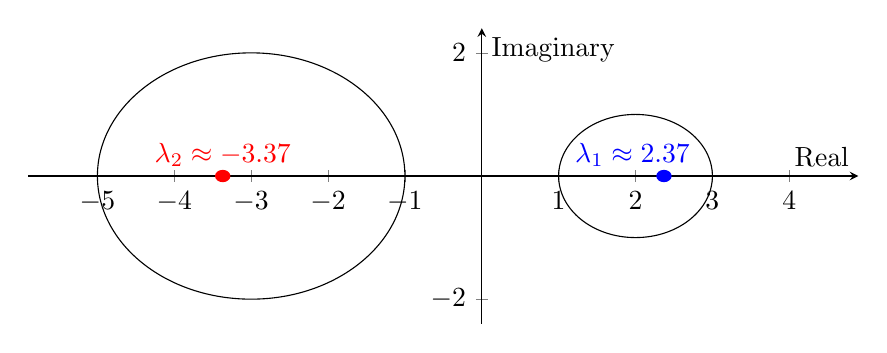
\begin{tikzpicture}
    \begin{axis}[axis lines=middle,
                 xlabel=Real,
                 ylabel=Imaginary,
                 width=\textwidth,
                 height=0.44\textwidth,
                 enlargelimits,
                 xmin=-5,xmax=4,
                 ymin=-2,ymax=2]
      \draw (axis cs:2,0) circle (1);
      \draw (axis cs:-3,0) circle (2);
      \fill[red] (axis cs:-3.37,0) circle[radius=0.1] node[above]
        {\( \lambda_2 \approx -3.37 \)};
      \fill[blue] (axis cs:2.37,0) circle[radius=0.1] node[above,xshift=-0.4cm]
        {\( \lambda_1 \approx 2.37 \)};
    \end{axis}
  \end{tikzpicture}
\end{center}

\subsubsection*{Example}
\begin{align*}
  A &= \begin{bmatrix}1 & -3 \\ 2 & 3\end{bmatrix} \\
  \det(A-\lambda I) &= 0 \\
  (1-\lambda)(3-\lambda)+6 &= 0 \\
  \lambda^2-4\lambda+9 &= 0 \\
  \lambda &= \frac{4+\pm\sqrt{16-36}}{2} \\
  &= 2\pm i\sqrt{5}
\end{align*}
\begin{center}
  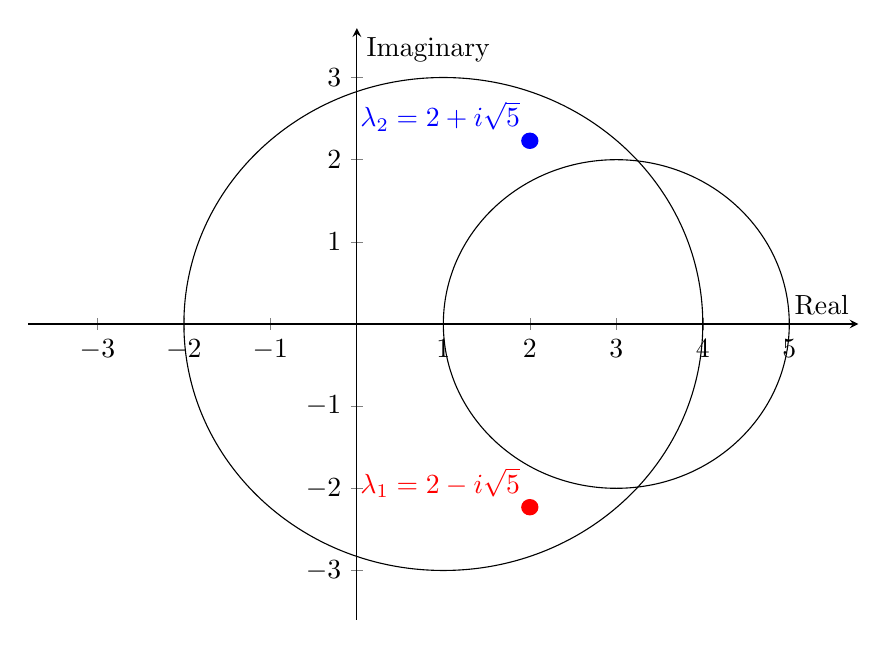
\begin{tikzpicture}
    \begin{axis}[axis lines=middle,
                 xlabel=Real,
                 ylabel=Imaginary,
                 width=\textwidth,
                 height=0.75\textwidth,
                 enlargelimits,
                 xmin=-3,xmax=5,
                 ymin=-3,ymax=3]
      \draw (axis cs:1,0) circle (3);
      \draw (axis cs:3,0) circle (2);
      \fill[red] (axis cs:2,-2.23) circle[radius=0.1] node[above left]
        {\( \lambda_1 = 2-i\sqrt{5} \)};
      \fill[blue] (axis cs:2,2.23) circle[radius=0.1] node[above left]
        {\( \lambda_2 = 2+i\sqrt{5} \)};
    \end{axis}
  \end{tikzpicture}
\end{center}

\subsection*{Proof}
Let \( A\vec{x} = \lambda\vec{x} \). Let \( x_i \) be the entry of \( \vec{x} \)
with the largest absolute value.
\begin{align*}
  \begin{bmatrix}a_{i1} & a_{i2} & \dots & a_{in}\end{bmatrix}
  \begin{bmatrix}x_1 \\ x_2 \\ \vdots \\ x_n\end{bmatrix} &= \begin{bmatrix}
    \vdots \\ \lambda x_i \\ \vdots
  \end{bmatrix} \\
  \sum_{j=1}^na_{ij}x_j &= \lambda x_i \\
  \sum_{j\ne i}a_{ij}x_j &= \lambda x_i-a_{ii}x_i
\end{align*}
\begin{align*}
  \lambda-a_{ii} &= \frac{1}{x_i}\sum_{j\ne i}a_{ij}x_j \\
  \|\lambda-a_{ii}\| &= \|\frac{1}{x_i}\sum_{j\ne i}a_{ij}x_j\| \\
  &= \frac{1}{\|x_i\|}\|\sum_{j\ne i}a_{ij}x_j\|
\end{align*}
Recall that the Triangle Inequality states:
\[ \|z+w\| \le \|z\|+\|w\| \]
\begin{align*}
  \|\lambda-a_{ii}\| &\le \frac{1}{\|x_i\|}\sum_{j\ne i}\|a_{ij}\|\|x_j\| \\
  &\le \sum_{j\ne i}\|a_{ij}\|
\end{align*}
This proof summarizes the essence of the theorem of Gerschgorin disks in that
all the eigenvalues of a matrix are contained with the Gerschgorin disk radii.

\begin{center}
  You can find all my notes at \url{http://omgimanerd.tech/notes}. If you have
  any questions, comments, or concerns, please contact me at
  alvin@omgimanerd.tech
\end{center}

\end{document}
